%!TEX root = ../thesis.tex
% ******************************* Thesis Appendix B ********************************

\chapter{Gradient estimation}
\label{app:grad_estim}
In order to perform gradient descent on the ELBO objective, we need to be able to evaluate its gradients with respect to parameters $\boldsymbol{\theta}$ and $\boldsymbol{\phi}$. Taking the gradient w.r.t generative parameters $\boldsymbol{\theta}$ is straightforward, because we can change the order of the expectation operator and the gradient, leaving us with
\begin{equation}
	\begin{aligned} 
		\nabla_{\boldsymbol{\theta}} \mathcal{L}_{\boldsymbol{\theta}, \boldsymbol{\phi}}(\mathbf{x}) &=\nabla_{\boldsymbol{\theta}} 	\mathbb{E}_{q_{\boldsymbol{\phi}}(\mathbf{z} \mid \mathbf{x})}\left[\log p_{\boldsymbol{\theta}}(\mathbf{x}, \mathbf{z})-\log q_{\boldsymbol{\phi}}(\mathbf{z} | \mathbf{x})\right] \\  & \simeq \nabla_{\boldsymbol{\theta}}\left(\log p_{\boldsymbol{\theta}}(\mathbf{x}, \mathbf{z})-\log q_{\boldsymbol{\phi}}(\mathbf{z} | \mathbf{x})\right) \\ &=\nabla_{\boldsymbol{\theta}}\left(\log p_{\boldsymbol{\theta}}(\mathbf{x}, \mathbf{z})\right) ,
	\end{aligned}
\end{equation}
where $\simeq$ denotes an unbiased estimator. This reversing of the order of operations is not possible when taking gradients w.r.t variational parameters $\boldsymbol{\phi}$ because the expectation $\mathbb{E}_{q_{\boldsymbol{\phi}}(\mathbf{z} | \mathbf{x})}$ is performed w.r.t the approximate posterior $q_{\boldsymbol{\phi}}(\mathbf{z} | \mathbf{x})$. The gradient could be estimated with a vanilla Monte Carlo estimator, but it has very high variance and is not practical~\cite{kingma2013auto}. 

The problem of stochastic gradient estimation of an expectation of a function is a well studied problem that transcends machine learning and has a variety of applications~\cite{chriss1997black, schrittwieser2020mastering}. Different estimators differ in from and their properties, variance being one of the most important. In their review~\cite{mohamed2020monte} Mohamed et al. categorise MC gradient estimators into three categories
\begin{enumerate}
	\item \emph{Score-function estimator}: The score function is a logarithm of a probability distribution w.r.t to distributional parameters. It can be used as a gradient estimator
	\begin{equation}
		\begin{aligned}
			\nabla_{\boldsymbol{\theta}} \mathbb{E}_{p_{\boldsymbol{\theta}}(\mathbf{x})}[f(\mathbf{x})] &=  \nabla_{\boldsymbol{\theta}} \int p_{\boldsymbol{\theta}}(\mathbf{x}) f(\mathbf{x}) d \mathbf{x} \\
			&= \mathbb{E}_{p_{\boldsymbol{\theta}}(\mathbf{x})}\left[f(\mathbf{x}) \nabla_{\boldsymbol{\theta}} \log p_{\boldsymbol{\theta}}(\mathbf{x})\right].
		\end{aligned}
	\end{equation}
	The score-function estimator is compatible with any cost function, it requires that the measure $p_{\boldsymbol{\theta}}(\mathbf{x})$ is differentiable and easy to sample. Very importantly it is applicable to both discrete and continuous distribution, but has a drawback of having high variance.
	
	\item \emph{Pathwise estimator}: Continuous distributions can be sampled either directly by generating samples from the distribution $p_{\boldsymbol{\theta}}(\mathbf{x})$ or indirectly, by sampling from a simpler base distribution $p(\boldsymbol{\epsilon})$ and transforming the variate through a deterministic path $g_{\boldsymbol{\theta}}(\boldsymbol{\epsilon})$. Using this, it is possible to move the source of randomness in such a way that the objective is differentiable. In essence this approach pushes the parameters of the measure into the cost function which is then differentiated. The estimator is
	\begin{equation}
		\begin{aligned}
			\nabla_{\boldsymbol{\theta}} \mathbb{E}_{p_{\boldsymbol{\theta}}(\mathbf{x})}[f(\mathbf{x})] 
			&=\nabla_{\boldsymbol{\theta}} \int p_{\boldsymbol{\theta}}(\mathbf{x}) f(\mathbf{x}) d \mathbf{x} \\
			&= \nabla_{\boldsymbol{\theta}} \int p(\boldsymbol{\epsilon}) f(g_{\boldsymbol{\theta}}(\boldsymbol{\epsilon})) d \boldsymbol{\epsilon} \\
			&= \mathbb{E}_{p(\boldsymbol{\epsilon})}\left[\nabla_{\boldsymbol{\theta}} f(g_{\boldsymbol{\theta}}(\boldsymbol{\epsilon}))\right].
		\end{aligned}
	\end{equation}
	\begin{figure}
		\centering
		\subfloat[Original]{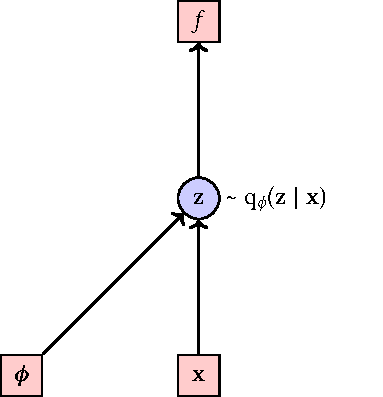
\includegraphics[height=7cm]{Appendix2/Figs/Vector/reparam_diagram.pdf}}
		\subfloat[Reparametrized]{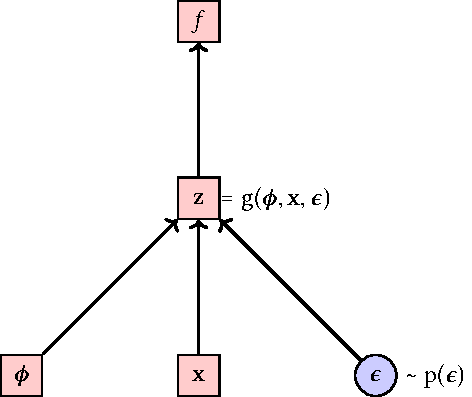
\includegraphics[height=7cm]{Appendix2/Figs/Vector/reparam_diagram2.pdf}}
		\caption[The reparametrization trick]{The reparametrization trick, adapted from~\cite{kingma2017variational}. The stochasticity of the $\mathbf{z}$ node is pushed out into a separate input to the same node, resulting in deterministic gradients w.r.t $\boldsymbol{\phi}$ through the node.}
		\label{fig:reparam}
	\end{figure}
	This was the gradient estimator originally used in the VAE implementation~\cite{kingma2013auto} there named as the \emph{reparametrization trick}, see also Figure~\ref{fig:reparam}. In many cases the transformation paths are so simple they can be implemented in one line of code, referred to as \emph{one-liners}. The pathwise-estimator can only be used on differentiable cost functions, but is easy to implement and crucially has lower variance than the score-function estimator. 
	
	\item \emph{Measure-valued gradient estimator}, which exploits the properties of signed-measures, is beyond the scope of this report.	
\end{enumerate}
Unbiased gradient estimation makes training on the ELBO objective possible. During training the VAE learns a mapping between a complicated observed space of $\mathbf{x}$ and the latent space of $\mathbf{z}$, which is usually defined to be relatively simple. The \emph{decoder} network or the \emph{generative} part of the VAE $p_{\boldsymbol{\theta}}(\mathbf{x} | \mathbf{z})$ learns to map from the latent space to the data space, while the \emph{inference} or \emph{encoder} network $q_{\mathbf{\phi}}(\mathbf{z}|\mathbf{x})$ approximates the true posterior $p_{\mathbf{\theta}}(\mathbf{z}|\mathbf{x})$ of this process, see Figure. 

